\documentclass[12pt]{article}%tamanho da fonte
\usepackage[utf8]{inputenc}
\usepackage[top=3cm, bottom=2cm, left=3cm, right=2cm]{geometry}%margens
\usepackage{indentfirst}%identação
\usepackage[portuguese]{babel}
\usepackage{setspace}%espaçamento
\usepackage{natbib}
\usepackage{graphicx}

\title{
Projeto de \LaTeX\\%titulo
Introdução à Computação\\
\Large Tema: Redes de Computadores - IF738\\%subtitulo
}
\author{Bruno Henrique dos Santos Marques}
\date{Data de entrega: 26/10/2020}

\begin{document}

\onehalfspacing %espaçamento de 1,5

\maketitle

\section{Introdu\c c\~ao}
\par As redes de computadores são definidas como o conjunto de equipamentos/computadores que possibilitam a troca entre si de informações, a partir de um sistema de comunicação.\citep{site}
\begin{figure}[h]
    \centering
    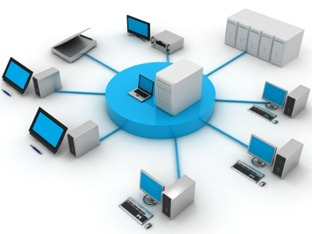
\includegraphics{introducao.jpg}
    \caption{Representação de uma rede de computadores\citep{introducao}}
\end{figure}
\par Esse sistema conecta todos os dispositivos através de um meio de transmissão e de um padrão que gerencia essas conexões, a comunicação e a transferencia dos dados entre os equipamentos/computadores.\citep{youtube}

\section{Relev\^ancia}

\subsection{Compartilhamento de dados}
\par Permite que cada computador pertecente à rede, possua acesso aos equipamento e dados existentes na organização.\citep{youtube}
\begin{figure}[h]
    \centering
    
\includegraphics[scale = 0.2]{datashare.jpg}
    \caption{Compartilhamento de dados\citep{datashare}}
\end{figure}
\subsection{Aumento da segurança dos dados}
\par Permite que existam cópias dos dados em diferentes máquinas. Assim, caso haja problemas com uma, as outras são capazes de garantir a acessibilidade dos dados. Além da substituição da operação de máquinas que possuem defeitos por outras operantes, garantindo a estabilidade do sistema, considerado ponto importante para diversas aplicações, como médicas, militares, econômicas, etc.\citep{youtube}
\begin{figure}[h]
    \centering
    
\includegraphics[scale = 0.7]{datasaving.jpg}
    \caption{Garante a existência dos dados\citep{datasaving}}
\end{figure}
\subsection{Redução de Custos}
\par Para que não seja necessária a obtenção e manutenção de uma máquina de grande porte e de custo elevado, é possível utilizar um grande número de microcomputadores que possuem menores custos, através da manipulação dos dados a partir de servidores de arquivos.\citep{youtube}
\begin{figure}[h]
    \centering
    
\includegraphics[scale = 0.2]{reduzircustos.jpg}
    \caption{Redução de custos\citep{reduzircustos}}
\end{figure}
\subsection{Redução do excesso de dados}
\par Com o compartilhamento dos dados, torna-se inexistente a necessidade de que cada computador no sistema possua uma cópia de cada arquivo.\citep{youtube}
\begin{figure}[h]
    \centering
    
\includegraphics[scale = 0.8]{limpezadados.jpg}
    \caption{Sem excesso de dados\citep{limpezadados}}
\end{figure}

\section{Rela\c c\~ao com outras disciplinas}

\subsection{IF678 - Infra-estrutura de Comunicação}
\par A disciplina IF678 - Infra-estrutura de Comunicação é considerada pré-requisito para a disciplina IF738 - Redes de Computadores.\citep{perfil}

\subsection{IF747 - Tópicos Avançados em Redes de Computadores}
\par A disciplina IF738 - Redes de Computadores é considerada pré-requisito para a disciplina IF747 - Tópicos Avançados em Redes de Computadores.\citep{perfil}

\bibliographystyle{plain}
\bibliography{ref}

\end{document}
